\chapter{Introducción específica} % Main chapter title

\label{Chapter2}

%----------------------------------------------------------------------------------------
%	SECTION 1
%----------------------------------------------------------------------------------------

En este capítulo se presentan los requerimientos del sistema y la planificación ejecutada. Además, se detallan las tecnologías utilizadas para el desarrollo tanto de software como de hardware del dispositivo primario y el dispositivo secundario.

\section{Detección de incendio}

Toda central de alarma de incendio debe notificar a los usuarios de la instalación de la presencia de un posible incidente y actuar en concordancia con el protocolo estipulado. Para ello generalmente el sistema segmenta los elementos de entrada y de salida según lo descrito en la figura \ref{fig:figura_a1}. Dividir el sistema facilita las conexiones, mantenimiento y respetar el estándar de la norma; en resumen la división consiste en: 

\begin{itemize}
\item  Lazo de detección: circuito eléctrico que contiene todos aquellos dispositivos asociados específicamente a la detección de posibles focos de incendio.
\item  Lazo de notificación: circuito eléctrico donde se encuentran aquellos equipos asociados a la notificación de un evento de alarma pueden ser parlantes, sirenas, luces estroboscópicas, entre otros.
\item  Interfaz con otros sistemas: relés programables ante diferentes eventos, un conjunto de interruptores que se utilizan para la notificación de eventos. Permite aislar el sistema y a la vez indicar de forma binaria el estado de un parámetro en particular.
\end{itemize}

\begin{figure}[h]
	\centering
	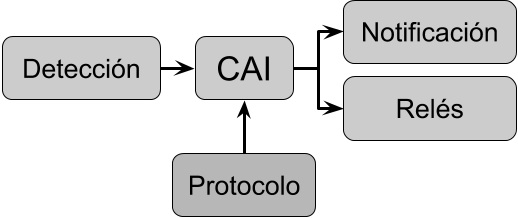
\includegraphics[scale=.45]{./Figures/Capitulo2/Figura_A.png}
	\caption{Diagrama de entradas y salidas de una central de alarma de incendio.}
	\label{fig:figura_a1}
\end{figure}

\section{Hardware}

Los componentes seleccionados para el sistema fueron seleccionados basados en los criterios de la sección \ref{criterios}. Existen tres componentes principales de hardware:  

\begin{itemize}
\item Raspberry Pi (dispositivo primario): es un computador de bajo costo que ejecuta un sistema operativo Linux \cite{RPI}. Tiene el tamaño de una tarjeta de crédito y cuenta con la capacidad de interactuar con componentes electrónicos externos mediante entradas y salidas de propósito general.

\begin{figure}[h]
	\centering
	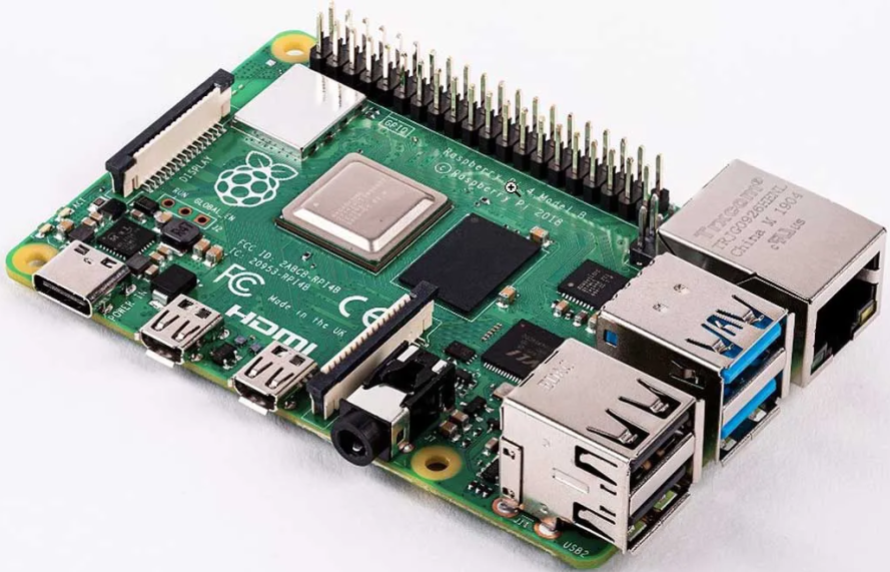
\includegraphics[scale=.25]{./Figures/Capitulo2/Figura_B.png}
	\caption{Raspberry Pi.}
	\label{fig:figura_b1}
\end{figure}


\item Node-MCU (dispositivo secundario): es un kit de desarrollo de bajo costo basado en el microcontrolador ESP8266 \cite{NODEMCU}. Algunas funcionalidades resaltantes son: regulador de tensión, entradas/salidas de propósito general y un  convertidor analógico digital. Permite el desarrollo de aplicaciones que requieren conexión a Internet de forma rápida, ya que incorpora conectividad Wi-Fi.

\begin{figure}[h]
	\centering
	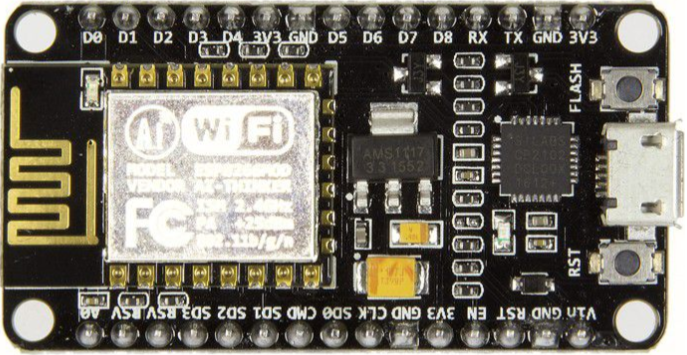
\includegraphics[scale=.25]{./Figures/Capitulo2/Figura_C.png}
	\caption{Node-MCU V3.0.}
	\label{fig:figura_c1}
\end{figure}

\item Nrf24l01 (comunicación inalámbrica): dispositivo transceptor \cite{rf24} con un protocolo incorporado de comunicación (Enhanced ShockBurst), que permite el diseño de sistemas comunicación inalámbrico con cualquier microcontrolador que cuente con comunicación SPI. Cuenta con parámetros configurables como frecuencia de trabajo (entre 2,400 - 2,4835 GHz), potencia y velocidad de transmisión de datos; lo que lo convierte en un sistema muy flexible para sistemas de bajo que requieran cumplir con requerimientos de bajo consumo.

\begin{figure}[h]
	\centering
	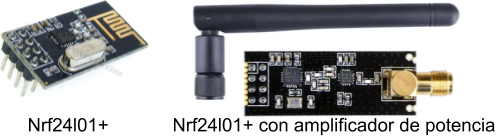
\includegraphics[scale=.65]{./Figures/Capitulo2/Figura_D.png}
	\caption{Nrf24l01+ y Nrf24l01+ con amplificador de potencia.}
	\label{fig:figura_d1}
\end{figure}
\end{itemize}

\section{Protocolos e interfaces}

Esta sección describe los protocolos que se utilizan internamente, junto con las plataformas y diferentes tecnologías empleadas por el sistema.      

\subsection{Protocolos de comunicación }
El sistema cuenta con diferentes equipos que se encuentran intercambiando información constantemente, por lo que se requiere de los siguientes protocolos que regulan la comunicación entre los dispositivos:

\begin{itemize}
\item  SPI (Serial Peripheral Interface): es un protocolo \cite{SPI} que permite la comunicación entre un dispositivo denominado “maestro” y varios dispositivos “esclavos”. El dispositivo maestro es responsable de iniciar la comunicación y define la tasa de transmisión basado en su señal de clock, es utilizado ampliamente entre microcontroladores y es el nexo que permite a los dispositivos primario y secundario interactuar con el transceptor Nrf24l01.

\item  TCP/IP + HTTP (Conexion a Internet ): el dispositivo primario requiere hacer la carga de información a un servidor web, para ello utiliza el protocolo TCP/IP para las capas de transporte y red, en conjunto con el protocolo HTTP para la capa de aplicación del estándar OSI.

\item  Enhanced Shockburst: un protocolo de comunicación basado en paquetes de datos que maneja de forma automática el empaquetado de la información, sincronización, transmisión y reconocimiento automático de transacciones. El protocolo soporta bidireccionalidad y se encuentra embebido en los elementos de la serie Nrf24lxx \cite{nrf24_protocol}.
\end{itemize}

\subsection{Interfaces}

El dispositivo primario otorga la información acerca del estado del sistema  al usuario. Requiere el desarrollo de Interfaces que permitan al usuario identificar fácilmente el estado de la instalación, al igual que un medio de acceso remoto sencillo que le permita acceder en cualquier momento.  

\begin{itemize}
\item Node-Red: herramienta de programación que provee una interfaz de desarrollo para servicios en línea \cite{node_red}. Funciona a través de programación en bloques y cuenta con diferentes integraciones con servicios de Internet, lo que facilita el desarrollo de interfaces de usuario personalizables.    

\item Firebase: es una plataforma de desarrollo de aplicaciones móviles \cite{firebase}. Brinda al usuario servicios de autenticación, bases de datos, almacenamiento, entre otros. Firebase permite realizar todas las conexiones necesarias para exportar la información desde el dispositivo primario a cualquier servicio de Internet, por ejemplo aplicaciones móviles o páginas web. 

\item Bases de datos con SQLite: SQLite es una biblioteca de funcionalidades reducidas que permite generar un motor de búsqueda SQL \cite{sqlite}. Las bases de datos generadas suelen utilizarse como contenedores de información para la transferencia organizada de información entre sistemas. EL uso de bases de datos permite registrar la información generada a partir de los análisis del dispositivo primario del sistema de detección de incendio.

\item MIT App Inventor: es un ambiente de programación en bloque que permite el diseño, simulación y construcción de aplicaciones para equipos móviles. Posee integración con Firebase por lo que con tan solo brindar los códigos de acceso, es posible acceder a la base de datos de cada proyecto.      
\end{itemize}

\section{Requerimientos}

A medida que se desarrollaba el sistema se realizaron reuniones mensuales con consultores y personal técnico de la empresa ISOLSE SRL. Los cambios más significativos consisten en facilitar el conexionado del sistema de monitoreo, eliminar la configuración manual y aprovechar los recursos del panel de control para el suministro eléctrico.   


\subsection{Normas de seguridad y garantía de servicio de ISOLSE SRL}
	\begin{enumerate}
	\item El sistema no deberá comprometer de ninguna manera el funcionamiento del sistema de detección de incendio.
	\item El sistema no deberá silenciar ni resetear los eventos presentes en el de detección de incendio de forma remota (basados en la norma NFPA punto 23.8.2.10 \cite{nfpa}). 
	\item El sistema de monitoreo remoto no transmitirá fallas internas al sistema de detección.
	\item El sistema de monitoreo deberá instalarse preferentemente en el mismo gabinete que la central de alarma.
	\end{enumerate}
	
\subsection{Funcionalidades comunes entre dispositivos primario y secundario}
	\begin{enumerate}
	\item Se realizará la adquisición del estado de los contactos secos.
		\begin{itemize}
		\item Contacto seco de falla en la central de alarma de incendio.
		\item Contacto seco de alarma en la central de alarma de incendio.
		\end{itemize}
	\item El suministro eléctrico deberá estar dentro del rango de los 12 a 24 VDC.
	\item Se deberá indicar el estado del sistema de detección de incendio a través de Leds, siguiendo la siguientes normas:
		\begin{itemize}
		\item  Verde en normal.
		\item  Amarillo para falla.
		\item  Rojo para alarma.
		\item  Rojo y amarillo para indicar alarma y falla presentes.				
		\end{itemize}
	\end{enumerate}
	
\subsection{Funcionalidades particulares del dispositivo primario}
	\begin{enumerate}
	\item Comunicación servidor web.
		\begin{enumerate}
		\item El sistema deberá tener la capacidad de transmitir información a un servidor web.
		\item La comunicación con el servidor web consistirá en enviar los siguientes datos al servidor web:
			\begin{itemize}
				\item La existencia de fallas en el sistema de detección de incendio. 	
				\item La existencia de alarmas en el sistema de detección de incendio.
				\item La presencia de fallas en el sistema de comunicación inalámbrica.
			\end{itemize}
		\item Se deberá establecer una comunicación con el servidor, ante un evento de cambio de estado del sistema de detección, en un intervalo de tiempo menor a 10 segundos.
		\item Se establecerá una comunicación inmediata con servidor web, si ocurre un cambio en el estado de los contactos secos.
		\item Se deberá establecer una comunicación con el servidor, ante un evento cambio de estado del sistema de comunicación inalámbrica, en un intervalo de tiempo menor a 10 segundos.
		\item Se generará un software encargado de generar y transmitir los paquetes de datos JSON.
		\item Se deberá establecer una prueba que permita verificar el funcionamiento de la comunicación con el servidor web. 
		\end{enumerate}
	\item Se registrarán al menos 500 eventos de forma local.
	\item Comunicación inalámbrica.
		\begin{enumerate}		
		\item Se realizará la adquisición del estado de los dispositivos secundarios a partir de los contactos secos monitoreados:
			\begin{itemize}
				\item Contacto seco de falla en la central de alarma de incendio.
				\item Contacto seco de alarma en la central de alarma de incendio.
			\end{itemize}	
		\item Se debe diseñar un mecanismo de recuperación ante fallas de comunicación inalámbrica.	
		\item Se realizará un software con la capacidad de recibir información por radiofrecuencia con hasta 3 dispositivos secundarios.
		\item Se establecerá una comunicación periódica con todos los dispositivos secundarios con una tasa de refresco de  al menos cada 2,5 s.
		\item Se deberá crear un software para controlar la secuencia de comunicación con dispositivos secundarios.
		\item Se deberá procesar los datos provenientes de dispositivos secundarios, para determinar los estados reales de la instalación.
		\item Se deberá establecer una prueba que permita verificar el funcionamiento de la comunicación por radiofrecuencia.
	\end{enumerate}
\end{enumerate}
\subsection{Funcionalidades particulares del dispositivo secundario}
	\begin{enumerate}	
		\item Se realizará un software con la capacidad de transmitir información por radiofrecuencia al dispositivo primario.
		\item Se establecerá una comunicación periódica con el dispositivo primario con una tasa de refresco de al menos cada 2,5 s.
		\item Se implementará un software con capacidad de reinicio, ante un total de 150 o más intentos fallidos de comunicación inalámbrica.
		\item Se deberá establecer una prueba que permita verificar el funcionamiento de la comunicación inalámbrica.
	\end{enumerate}
	
\subsection{Condiciones de trabajo}
	\begin{enumerate}
		\item Idealmente el sistema tendrá que estar resguardado dentro de la central de incendio, en caso contrario se requerirá una protección IP51.
	\end{enumerate}


\begin{comment}
\begin{enumerate}
\item Normas de seguridad y garantía de servicio de ISOLSE SRL.
	\begin{enumerate}
	\item El sistema no deberá comprometer de ninguna manera el funcionamiento del sistema de detección de incendio.
	\item El sistema no deberá silenciar ni resetear los eventos presentes en el de detección de incendio de forma remota. 
	\item El sistema de monitoreo remoto no transmitirá fallas internas al sistema de detección.
	\item En caso de corte del suministro eléctrico el sistema no deberá afectar de ninguna manera la autonomía de la central.
	\item El sistema de monitoreo deberá instalarse preferentemente en el mismo gabinete que la central de alarma.
	\end{enumerate}
\item Funcionalidades comunes entre dispositivos primario y secundario.
	\begin{enumerate}
	\item Se realizará la adquisición del estado de los contactos secos.
		\begin{itemize}
		\item Contacto seco de falla en la central de alarma de incendio.
		\item Contacto seco de alarma en la central de alarma de incendio.
		\end{itemize}
	\item El suministro eléctrico deberá estar dentro del rango de los 12 a 24 VDC.
	\item Se deberá indicar el estado del sistema de detección de incendio a través de Leds, siguiendo la siguientes normas:
		\begin{itemize}
		\item  Verde en normal.
		\item  Amarillo para falla.
		\item  Rojo para alarma.
		\item   Rojo y amarillo para indicar alarma y falla presentes.				
		\end{itemize}
	\end{enumerate}
\item Funcionalidades particulares del dispositivo primario.
	\begin{enumerate}
	\item Comunicación servidor web.
		\begin{enumerate}
		\item El sistema deberá tener la capacidad de transmitir información a un servidor web.
		\item La comunicación con el servidor web consistirá en enviar los siguientes datos al servidor web:
			\begin{itemize}
				\item La existencia de fallas en el sistema de detección de incendio. 	
				\item La existencia de alarmas en el sistema de detección de incendio.
				\item La presencia de fallas en el sistema de comunicación inalámbrica.
			\end{itemize}
		\item Se deberá establecer una comunicación con el servidor, ante un evento de cambio de estado del sistema de detección, en un intervalo de tiempo menor a 10 segundos.
		\item Se establecerá una comunicación inmediata con servidor web, si ocurre un cambio en el estado de los contactos secos.
		\item Se deberá establecer una comunicación con el servidor, ante un evento cambio de estado del sistema de comunicación inalámbrica, en un intervalo de tiempo menor a 10 segundos.
		\item Se generará un software encargado de generar y transmitir los paquetes de datos JSON.
		\item Se deberá establecer una prueba que permita verificar el funcionamiento de la comunicación con el servidor web. 
		\end{enumerate}
	\item Se registrarán al menos 500 eventos de forma local.
	\item Comunicación inalámbrica.
		\begin{enumerate}		
		\item Se realizará la adquisición del estado de los dispositivos secundarios a partir de los contactos secos monitoreados:
			\begin{itemize}
				\item Contacto seco de falla en la central de alarma de incendio.
				\item Contacto seco de alarma en la central de alarma de incendio.
			\end{itemize}	
		\item Se debe diseñar un mecanismo de recuperación ante fallas de comunicación inalámbrica.	
		\item Se realizará un software con la capacidad de recibir información por radiofrecuencia con hasta 3 dispositivos secundarios.
		\item Se establecerá una comunicación periódica con todos los dispositivos secundarios con una tasa de refresco de  al menos cada 2,5 s.
		\item Se deberá crear un software para controlar la secuencia de comunicación con dispositivos secundarios.
		\item Se deberá procesar los datos provenientes de dispositivos secundarios, para determinar los estados reales de la instalación.
		\item Se deberá establecer una prueba que permita verificar el funcionamiento de la comunicación por radiofrecuencia.
	\end{enumerate}
\end{enumerate}
\item Funcionalidades particulares del dispositivo secundario.
	\begin{enumerate}	
		\item Se realizará un software con la capacidad de transmitir información por radiofrecuencia al dispositivo primario.
		\item Se establecerá una comunicación periódica con el dispositivo primario con una tasa de refresco de al menos cada 2,5 s.
		\item Se implementará un software con capacidad de reinicio, ante un total de 150 o más intentos fallidos de comunicación inalámbrica.
		\item Se deberá establecer una prueba que permita verificar el funcionamiento de la comunicación inalámbrica.
	\end{enumerate}
\item Condiciones de trabajo.
	\begin{enumerate}
		\item Idealmente el sistema tendrá que estar resguardado dentro de la central de incendio, en caso contrario se requerirá una protección IP51.
	\end{enumerate}
\end{enumerate}
\end{comment}
 
%\subsection{Uso del Nrf24l01+}
%\begin{itemize}
%\item  Nrf24l01 amplificador de potencia con reducción de ruido y antena.
%\item  Nrf24l01 + anten
%\item  Fuente de poder Canakit micro USB 2,5 A con filtro de ruido.
%\item Adaptador 120-240 VA a 5V DC USB.
%\end{itemize}

%\begin{figure}[ht]
%	\centering
%	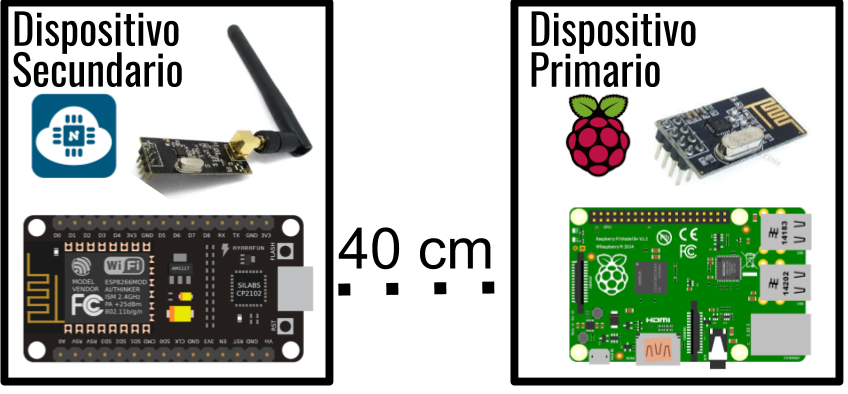
\includegraphics[scale=.45]{./Figures/Capitulo4/Figura_A.png}
%	\caption{Esquema utilizado para el ensayo del Nrf24l01+.}
%	\label{fig:figura_a}
%\end{figure}
%\ref{fig:figura_a}
